\chapter{Introducere}

\section{Motivația unui sistem de analiză a jocurilor de tenis de masă}
Arbitrajul unui meci oficial de tenis de masă este realizat de către un arbitru, responsabil de luarea deciziilor privind punctele, greșelile și respectarea regulamentului, alături de un arbitru asistent care ajută la numărarea atingerilor fileului, controlează timpul și alte detalii tehnice. Mai mult, în cadrul Campionatelor Mondiale ITTF, numărul meselor de tenis care susțin jocuri în paralel variază între 40 și 60 la început, iar în faza finală se utilizează o singură masă.

 Implementarea unui sistem de analiză a jocurilor de tenis de masă pentru reducerea numărului de decizii eronate se dovedește a fi rentabilă în cadrul unui campionat deoarece utilizarea arbitrilor scade exponențial și există responsabilități simple care pot fi îndeplinite de un sistem.

 Structura și regulile unui meci de tenis de masă sunt standardizate în cadrul campionatelor, astfel încât anumite informații precum existența celor doi jucători de-o parte și de alta a mesei, forma dreptunghiulară a mesei și culoarea mingii de tenis de masă, pot reprezenta o bază a sistemului nostru automat de analiză.

 
\section{Scopul lucrării}
Această lucrare are ca scop dezvoltarea unui sistem automat capabil să detecteze și să analizeze elementele esențiale ale unui joc de tenis de masă. Componentele identificate sunt organizate în trei categorii principale:

\begin{itemize}
    \item \textbf{Elemente statice}: masa și fileul de tenis de masă;  
    \item \textbf{Elemente dinamice}: mingea și paletele jucătorilor; 
    \item \textbf{Evenimente din joc}: traiectoria mingii, punctele de contact cu masa și loviturile de retur.  
\end{itemize}

\begin{figure}[H]
    \centering
    \begin{subfigure}[b]{0.48\linewidth}
        \centering
        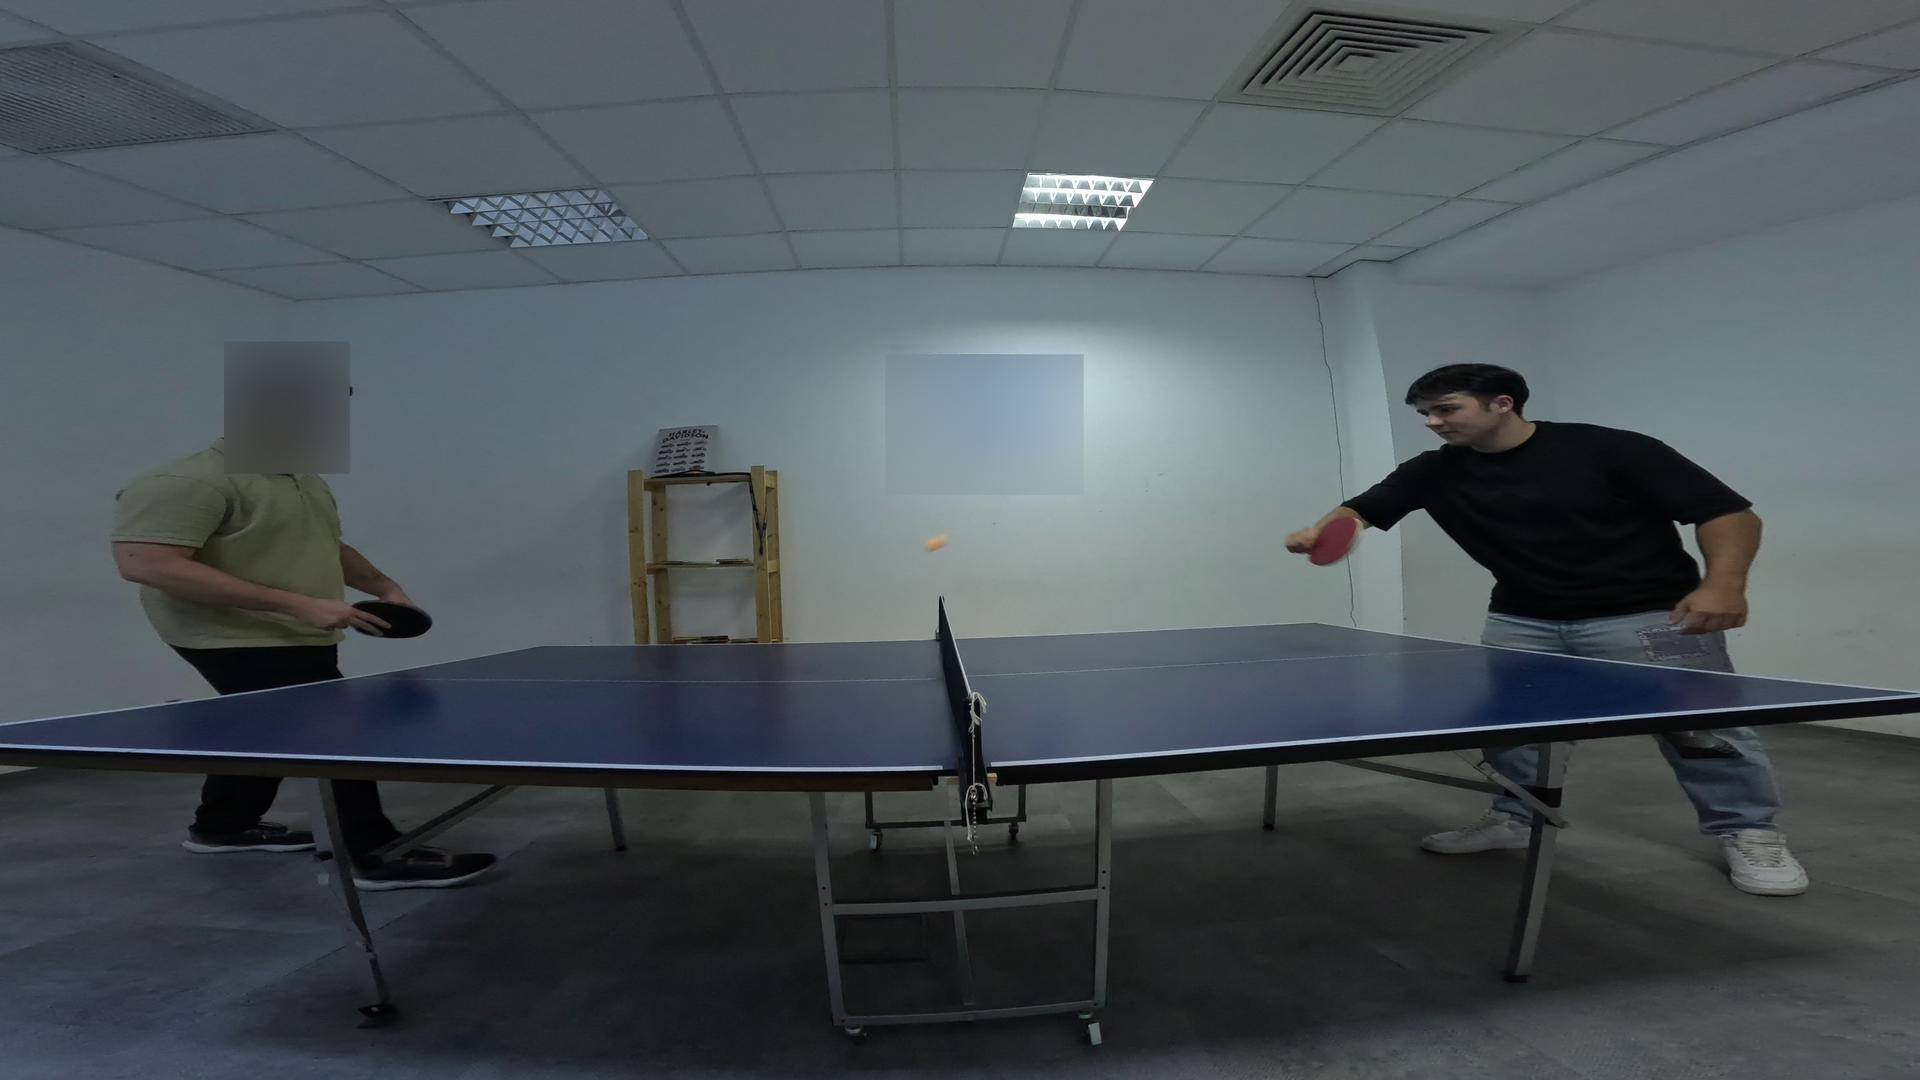
\includegraphics[width=\linewidth]{images/cst-pre.jpg}
        \caption{Cadru neprocesat.}
        \label{fig:cst-pre}
    \end{subfigure}
    \hfill
    \begin{subfigure}[b]{0.48\linewidth}
        \centering
        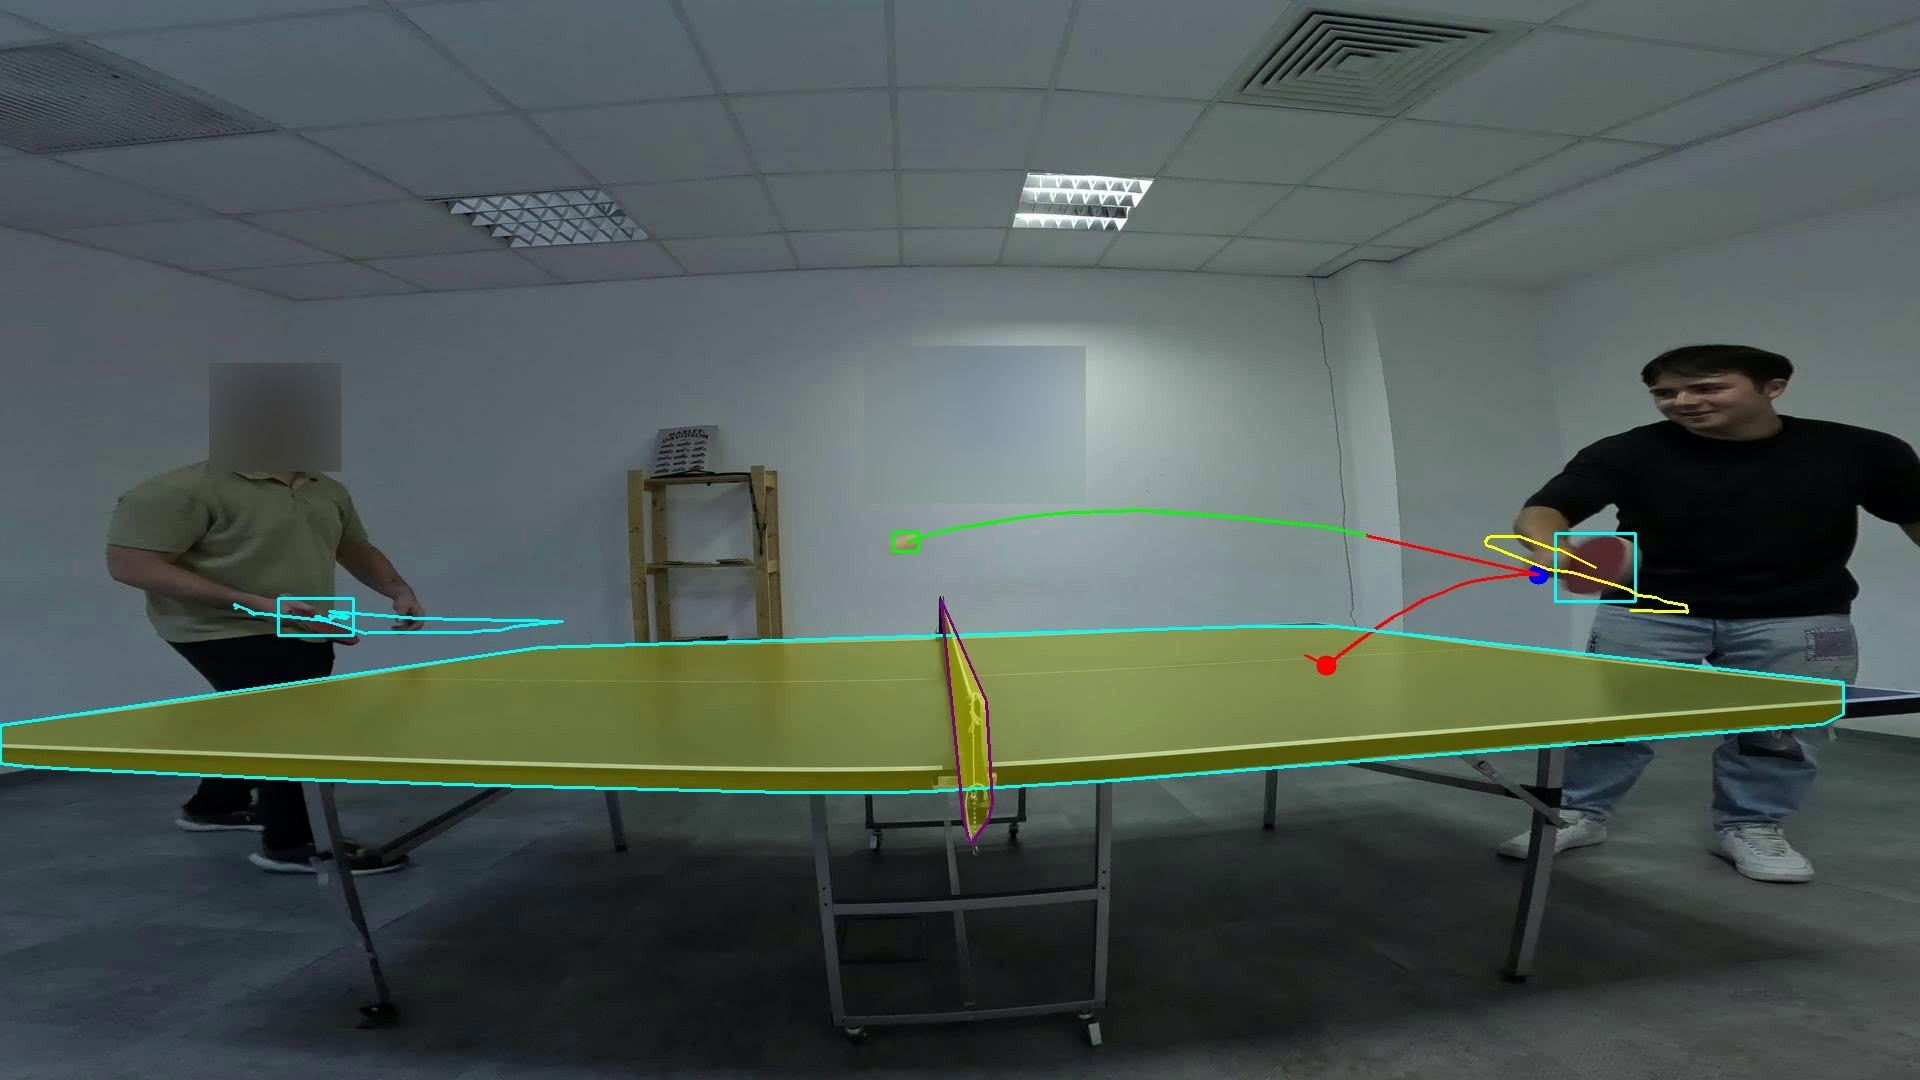
\includegraphics[width=\linewidth]{images/cst-post.jpg}
        \caption{Cadru procesat.}
        \label{fig:cst-post}
    \end{subfigure}

    \vspace{0.5cm} 

    \begin{subfigure}[b]{0.48\linewidth}
        \centering
        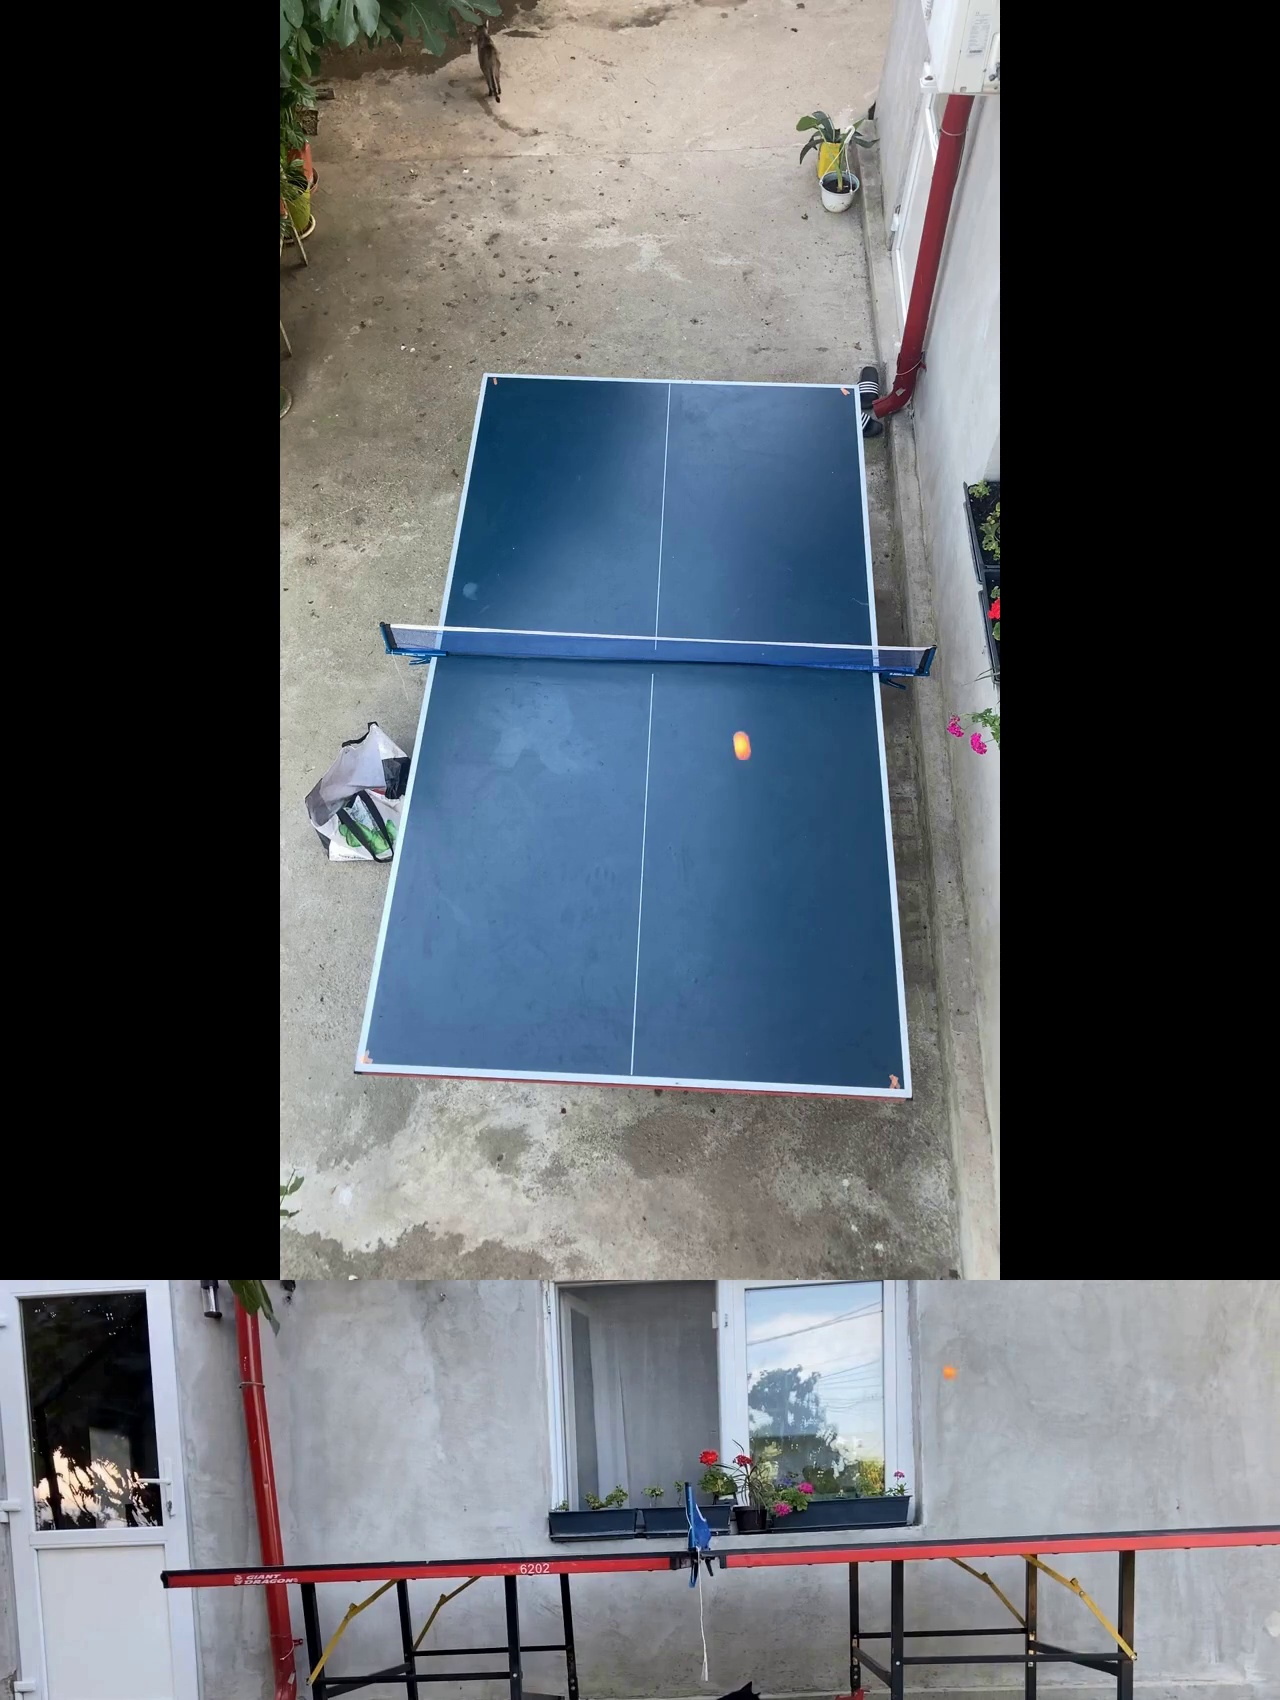
\includegraphics[width=\linewidth]{images/double-pre.jpg}
        \caption{Cadru neprocesat - vedere stereoscopică.}
        \label{fig:double-pre}
    \end{subfigure}
    \hfill
    \begin{subfigure}[b]{0.48\linewidth}
        \centering
        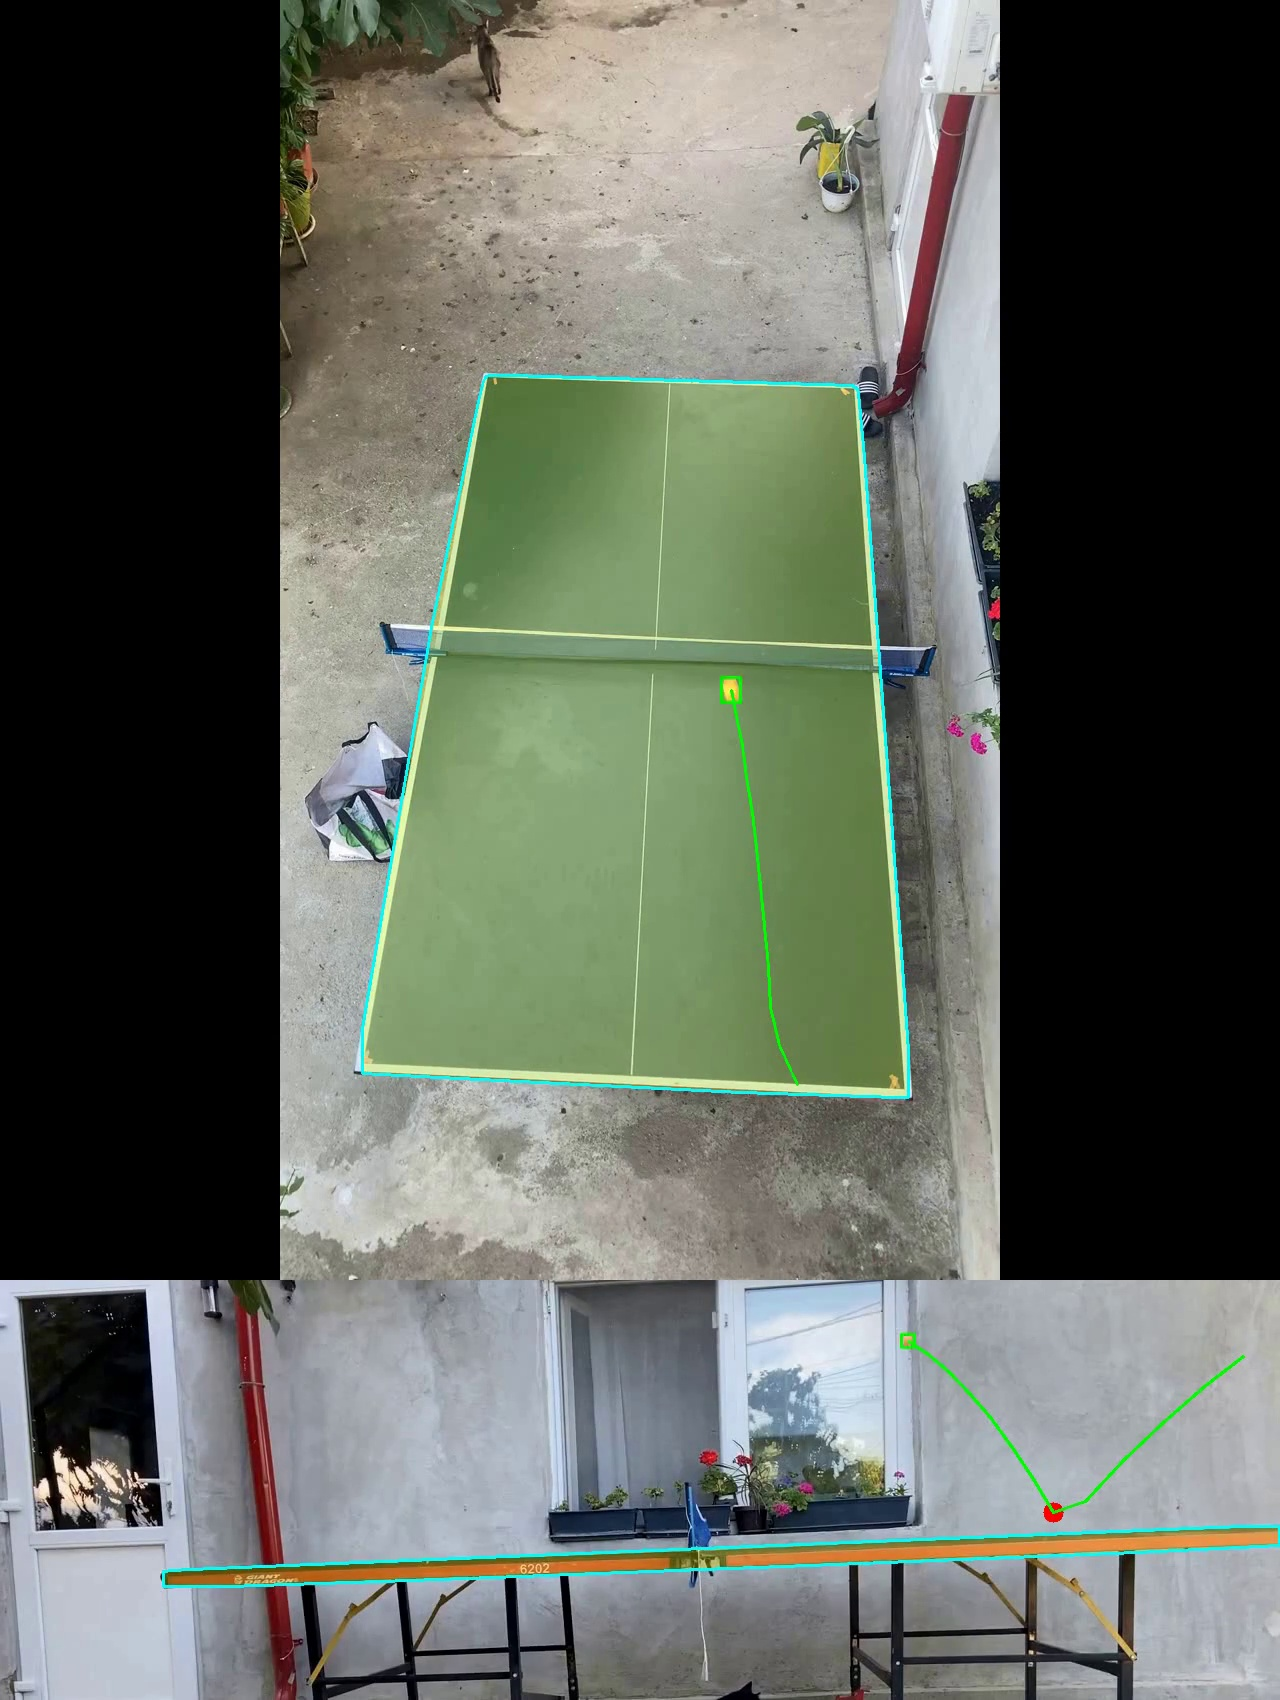
\includegraphics[width=\linewidth]{images/double-post.jpg}
        \caption{Cadru procesat - vedere stereoscopică.}
        \label{fig:double-post}
    \end{subfigure}

    \vspace{0.5cm}

    \begin{subfigure}[b]{0.48\linewidth}
        \centering
        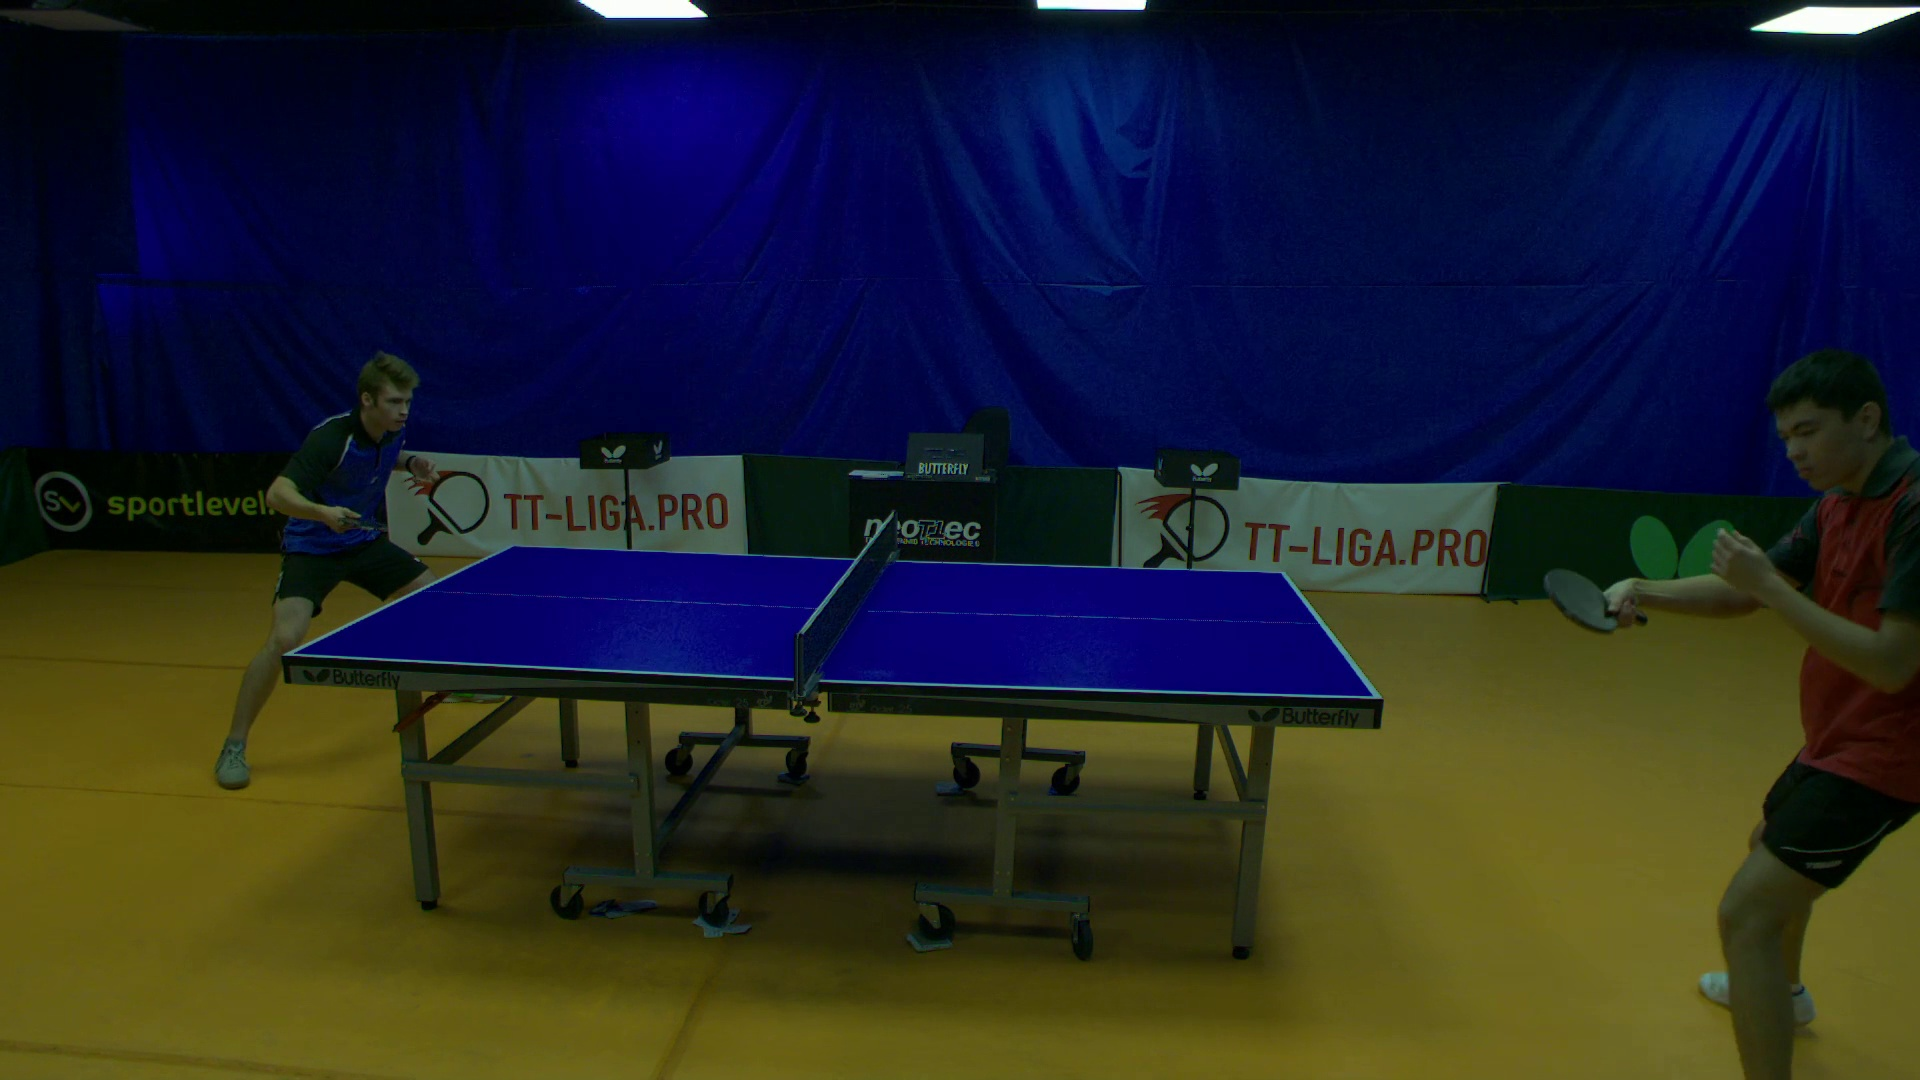
\includegraphics[width=\linewidth]{images/osai-pre.jpg}
        \caption{Cadru neprocesat - TTNet.}
        \label{fig:osai-pre}
    \end{subfigure}
    \hfill
    \begin{subfigure}[b]{0.48\linewidth}
        \centering
        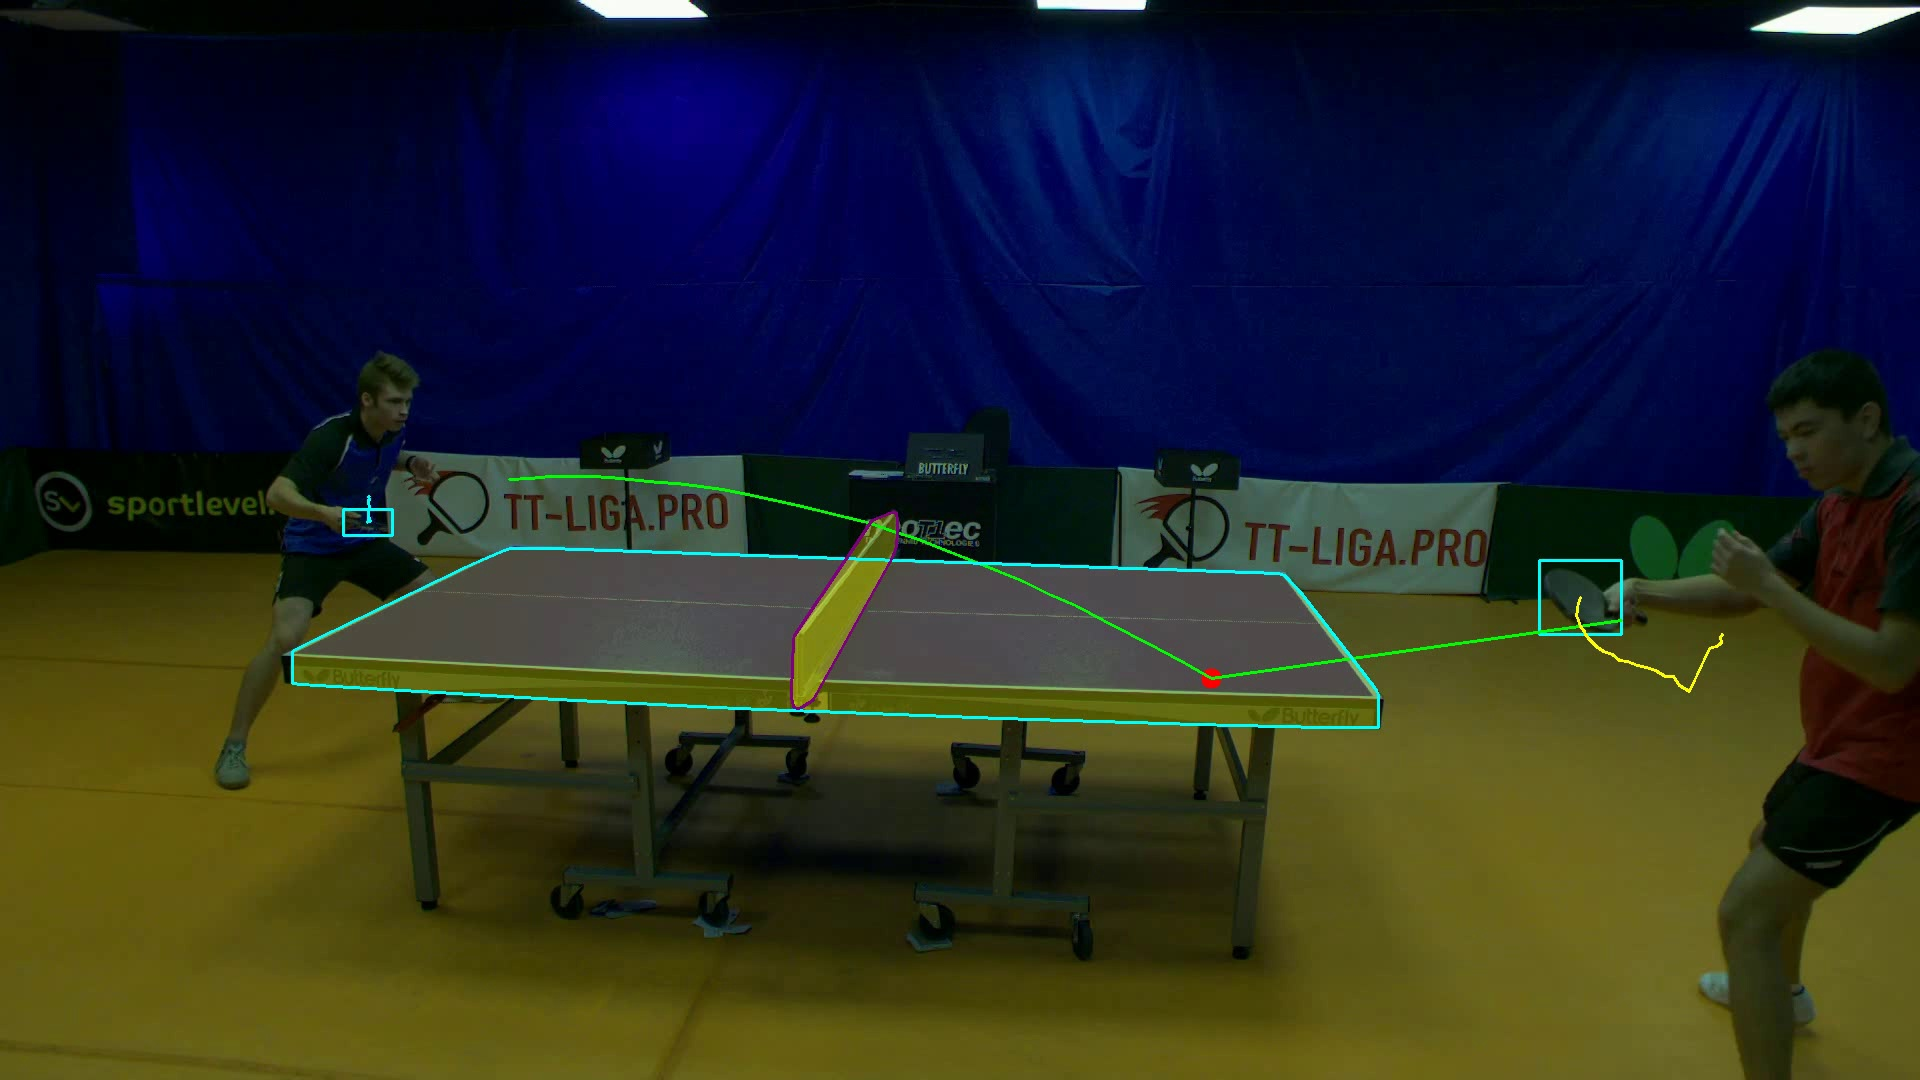
\includegraphics[width=\linewidth]{images/osai-post.jpg}
        \caption{Cadru procesat - TTNet.}
        \label{fig:osai-post}
    \end{subfigure}
    
    \caption{Compararea cadrelor neprocesate și procesate de către sistemul propus.}
    \label{fig:comparatie-cadre}
\end{figure}



În scopul unei interpretări vizuale clare, am adoptat o schemă de culori specifică, ilustrată în Figura \ref{fig:comparatie-cadre}, care compară cadrele neprocesate cu cele rezultate din sistemul propus:
\begin{itemize}
    \item Masa de joc va fi evidențiată cu un \textbf{chenar galben cu bordură albastră};
    \item Traiectoria mingii va fi \textbf{marcată cu verde};
    \item Paletele vor fi evidențiate cu un \textbf{chenar albastru}, iar traiectoriile vor fi de culoare \textbf{albastră}, respectiv \textbf{galbenă}, în funcție de poziția jucătorului;
    \item Evenimentele de săritură ale mingii vor fi \textbf{marcate cu roșu}, iar loviturile de retur vor fi \textbf{indicate cu puncte albastre}.
\end{itemize}


Pentru atingerea scopului propus, această lucrare urmărește realizarea următoarelor obiective:
\begin{enumerate}
    \item Detectarea elementelor cheie care stau la baza tenisului de masă: mingea, paletele, masa, fileul și evenimentele de săritură și retur;
    \item Evaluarea acurateței detectării mingii și a evenimentelor. Performanța metodei propuse va fi comparată cu o altă lucrare din literatura de specialitate;
    \item Adaptarea algoritmului în diferite scenarii;
    \item Optimizarea vitezei de procesare pentru a permite analiza cadrelor în timp real;
    \item Implementarea unei metode de analiză a coordonatelor mingii de tenis de masă într-un spațiu tridimensional.
\end{enumerate}




